\scanpage{22}
\begin{flushright}
\uline{tap\unsure{i|\^{\i}}s Quillen} (Notes du 6.9.68)
\end{flushright}

1.\quad Catégories formelles.

Catégorie formelle \begin{tabular}[b]{@{}l@{}}\inserted{$\mathcal C$}\\[-0.4ex]\begin{tikzpicture}[x=0.23cm,y=0.23cm,baseline] \draw (0,-.45) .. controls (.04,.08) and (.15,.55) .. (.28,.91) .. controls (.37,1.15) and (.51,1.28) .. (.45,1.49); \end{tikzpicture}\end{tabular} ``sur $X_0$'' i.e. dont l\unsure{e|es} 'objet des objets est le schéma $X_0$ (\unsure{re}gardé comme \deleted{i\unsure{n}d\unsure{-}} schéma formel i.e. \uline{ind-schém\unsure{a|.}} particulier).

Revient à la donnée d'un pro-Anneau strict \begin{tabular}[b]{@{}l@{}}\inserted{``admissible''}\\[-0.4ex]\begin{tikzpicture}[x=0.23cm,y=0.23cm,baseline] \draw (0,-.45) -- (0,.12) .. controls (0,.3) and (.13,.37) .. (.35,.37) .. controls (1.15,.35) and (2.35,.29) .. (3.04,.31) .. controls (3.25,.32) and (3.4,.38) .. (3.38,.58); \end{tikzpicture}\end{tabular} $A$ sur $X_0$, augmenté vers $\underline O_{X_0}$ {\reversemarginpar\margin{%
\diagram{\begin{tikzcd}[ampersand replacement=\&,row sep=large]
X_2 \arrow[d,shift right=4.4ex] \arrow[d,shift right=2.2ex] \arrow[d] \\
X_1 \arrow[u,shift right=2.3ex,bend right=9] \arrow[u,shift right=4.4ex,bend right=9] \arrow[d,shift right=2ex] \arrow[d] \\
X_0 \arrow[u,shift right=2.4ex,bend right=10]
\end{tikzcd}}
}}, l'idéal d'augmentation étant idéal de definition, avec deux structures de $\underline O_{X_0}$-modules (g. et dr), et \unsure{s|d} un hom. \begin{tabular}[b]{@{}l@{}}\inserted{de bi-$\underline O_{X_0}$-proanneaux}\\[-0.4ex]\begin{tikzpicture}[x=0.23cm,y=0.23cm,baseline] \draw (0,-.3) .. controls (-.13,.07) and (.02,.24) .. (.27,.26) .. controls (1.03,.34) and (1.65,.51) .. (2.45,.47) .. controls (3.2,.44) and (3.76,.28) .. (3.91,.46) .. controls (3.97,.54) and (3.92,.59) .. (3.94,.63); \end{tikzpicture}\end{tabular} $\unsure{A}\xrightarrow{\Delta}A_{\mathrm{dr}}\otimes_{\underline O_{X_0}}{}_{\mathrm g}A\ \deleted{\unsure{\longrightarrow}}$, satisfaisant des axiomes évidents a) ``associativité'' de $\Delta$ b) unitarité g. et dr. \unsure{vis|vs} à \unsure{vis|vs} de l'augmentation. [Cela sera-t-il nécessairement \uline{u}\unsure{n|ne} \deleted{catégorie} \uline{groupoïde} formel, i.e. y-aura-t-il une \uline{symétrie} $s$ de $A$, jouant vis-à-vis de $\Delta$ et de l'augmentation $\varepsilon$ le rôle d'\unsure{un|u} passage à l'inverse ?]

On pose $\Omega_{\mathcal C}={}$faisceau conormal de $X_0$ dans $X_1$ ; à priori c'est un \unsure{pro-|p-}faisceau qu. ch. sur $X_0$, mais dans le cas où $A$ est $I$-\uline{adique} [$I$ l'idéal d'augmentation] c'est un module qu. ch. ordinaire.

On définit alors sur $\overset{*}{\bigwedge}\Omega$ une différentielle d'anneau gradué \begin{tabular}[b]{@{}l@{}}\inserted{$d:d_{\mathcal C}$}\\[-0.4ex]\begin{tikzpicture}[x=0.23cm,y=0.23cm,baseline] \draw (.7,.85) .. controls (1.03,.91) and (.64,.45) .. (.29,.2) .. controls (.06,.06) and (-.12,-.01) .. (-.11,-.33); \draw (-.21,-.21) -- (-.11,-.33) -- (-.03,-.2); \end{tikzpicture}\end{tabular} Sa valeur sur $\overset{0}{\bigwedge}\Omega=\underline O_{X_0}$ est
\[
df=\mathrm{pr}_2^{*}(f)-\mathrm{pr}_1^{\unsure{\alpha|*|d}}(f)\mod I^2
\]

{\reversemarginpar\margin{\uline{n'intervien\unsure{dra|t}}\\\uline{pas plus bas}}}
\noindent\begin{tabular}{@{}p{0.025\linewidth}@{\hspace{0.5em}}p{0.94\linewidth}@{}}
\raisebox{-0.2em}{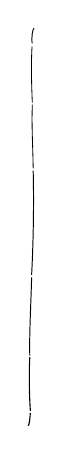
\begin{tikzpicture}[x=0.18cm,y=0.54cm,baseline=(current bounding box.north)]
\draw[line width=0.35pt] (0.14,0) .. controls (0.03,-0.03) and (-0.04,-0.2) .. (0,-0.36);
\draw[line width=0.3pt] (0,-0.43) .. controls (-0.08,-0.85) and (-0.03,-1.4) .. (0.02,-1.75);
\draw[line width=0.3pt] (0.02,-1.8) .. controls (-0.04,-2.3) and (0.06,-2.8) .. (0.08,-3.3);
\draw[line width=0.35pt] (0.08,-3.35) .. controls (0.14,-4.2) and (0.08,-5.1) .. (-0.03,-5.8);
\draw[line width=0.35pt] (-0.03,-5.86) .. controls (-0.08,-6.5) and (-0.2,-7.2) .. (-0.16,-7.7);
\draw[line width=0.4pt] (-0.16,-7.74) .. controls (-0.23,-8.2) and (-0.18,-8.7) .. (-0.12,-9.0);
\draw[line width=0.4pt] (-0.12,-9.05) .. controls (-0.16,-9.22) and (-0.2,-9.32) .. (-0.27,-9.35);
\end{tikzpicture}} &
\uline{Sorite à développer} : $A=(A_\alpha)$, regardons $A_\alpha$ comme module pour la structure gauche, alors l'application $f\longmapsto\mathrm{pr}_{\unsure{2|\alpha}}^{\unsure{*}}(f):\underline O_{\unsure{X_0|X}}\mathbin{-}A_\alpha$ est un op. diff. [d'ordre $n$ si $I_\alpha^{n+1}=0$], et par suite tte \deleted{f\unsure{orme} li} section de $\underline{\mathrm{Hom}}_{\underline O_{\unsure{X_0|X}}}(A_\alpha,\underline O_{\unsure{X_0|X}})=\underline{\mathscr D}_\alpha^{\mathcal C}$ definit un op. différentiel dans $\underline O_{\unsure{X_0|X}}$. Alors $\mathscr D_{\unsure{0|\mathcal C|\mathrm g}}^{\mathcal C}=\underline{\lim}_\alpha\mathscr D_\alpha^{\mathcal C}$ est un faisceau d'algèbres \begin{tabular}[b]{@{}l@{}}\inserted{unitaires \unsure{nc.|m.|n.}}\\[-0.4ex]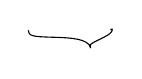
\begin{tikzpicture}[x=0.23cm,y=0.23cm,baseline] \draw (0,.35) .. controls (0,.03) and (.35,.01) .. (1.1,-.02) .. controls (2.05,-.05) and (3.01,-.05) .. (3.35,-.43) .. controls (3.54,-.75) and (3.38,-.65) .. (3.44,-.43) .. controls (3.65,-.23) and (4.47,.03) .. (4.61,.29) .. controls (4.69,.43) and (4.59,.47) .. (4.54,.38); \end{tikzpicture}\end{tabular} [\unsure{grâce à|gr. à :} l'application $\Delta$], qui s'envoie dans le faisceau des op différentiels [qui correspond
\end{tabular}

{\reversemarginpar\margin{21}}

